\section{Theoretische und technische Grundlagen}

\subsection{Datenstrukturen}
\subsubsection{Graph}
Um das kürzeste-Wege-Problem zu lösen, muss zunächst das reale Straßennetz in eine abstrakte Form
gebracht werden. Hierzu wird das Straßennetz als Graph modelliert. Ein Graph $G = (V,E)$ besteht aus
einer Menge von Knoten V und einer Menge von Kanten E. Jede Kante $e = (u,v)\in E$ verbindet zwei
Knoten $u,v \in V$. Knoten bilden Kreuzungen ab und Kanten Straßensegmente zwischen zwei Kreuzungen.
Ein Graph kann als gerichtet oder ungerichtet definiert werden. Bei einem ungerichteten  Graphen
sind die Kanten bidirektional und können in beide Richtungen durchlaufen werden, während bei einem
gerichteten Graphen die Kanten nur in eine Richtung durchlaufen werden können.\\

Der Graph in dieser Arbeit ist gerichtet und gewichtet. Die Kantenrichtung spiegelt dabei die
Richtung des Verkehrs wieder, \dH sie gibt an, ob eine Straße in einer bestimmten Richtung befahren
werden darf oder nicht. Zusätzlich wird auf jede Kante eine Kostenfunktion angewandt, die dann ein
Gewicht $w(e)$ festgelegt. In der Routenplanung ist normalerweise nicht die kürzeste Strecke von
Interesse, sondern die Strecke mit der kürzesten Reisezeit. Diese lässt sich aus der
Länge des Straßensegments \emph{S} und der maximal erlaubten Geschwindigkeit \emph{V} auf dieser
Straße $t = \frac{V}{S}$ in Sekunden berechnen.\\

Es gibt generell zwei Möglichkeiten, einen Graphen als Datenstruktur darzustellen. Eine davon ist
die Verwendung von Adjazenzlisten. Dabei wird für jeden Knoten $u \in V$ eine Liste der benachbarten
Knoten bzw. ausgehenden Kanten $e(u,v) \in E$ gespeichert. Die Summe der Länge aller Adjazenzlisten
in einem gerichteten Graph entspricht der Anzahl an Kanten $|E|$, bzw. $2|E|$ in einem ungerichteten
Graph. Der Speicherverbrauch für die Adjazenzliste ist damit $\Theta(|V| + |E|)$ \cite{intro.algo}.

Die zweite Möglichkeit ist die Verwendung einer Adjazenzmatrix. Hier wird eine zweidimensionale
Matrix der Größe $|V| \times |V|$ verwendet, bei der die Zeilen und Spalten den Knoten entsprechen.
Der Eintrag an Position $(i,j)$ in der Matrix gibt an, ob eine Kante zwischen den Knoten $i$ und $j$
existiert. Unabhängig von der Anzahl an Kanten ist der Speicherverbrauch $\Theta(|V|^2)$
\cite{intro.algo}. Ein Beispiel für beide Darstellungen anhand eines einfachen Graph befindet sich
in Abbildung~\ref{fig:graph_ex1}.\\

Für diese Arbeit werden Adjazenzlisten verwendet, da zum einen Straßennetze dünne Graphen sind ($|E|
    << |V|^2$), und damit die Speichereffizienz gegenüber einer Adjazenzmatrix deutlich effizienter
ist. Zum anderen ist für es wichtig, für den Aufbau der \ac{CHs} und der Suche, schnell auf alle
Nachbarn eines Knotens zuzugreifen zu können. Der Zugriff auf
eingehende Kanten ist allerding nur sehr aufwendig  möglich, wird  aber für den Aufbau der
Kontraktionshierarchien benötigt. Das Problem lässt sich jedoch lösen indem auch
Adjazenzlisten für alle eingehenden Kanten eines Knotens angelegt werden. Damit erhöht sich der
Speicherverbrauch auf $\Theta(|V| + 2|E|)$, was aber immer noch deutlich effizienter ist als
eine Darstellung als Adjazenzmatrix.%\todo{Ref genaue Datenstruktur?}

% \font\nullfont=cmr10
\begin{figure}[H]
    \centering
    \begin{subfigure}{1.0\textwidth}
        \centering
        \begin{tikzpicture}
            \Vertices[color=gray!90!blue]{data/graphs/ex1/vertices.csv}
            \Edges{data/graphs/ex1/edges.csv}
        \end{tikzpicture}
        \caption{}
    \end{subfigure}
    \\[3ex]
    \begin{subfigure}[b]{0.3\textwidth}
        \centering
        \begin{blockarray}{c|ccccc}
            & A & B & C & D & E \\
            \BAhline
            \begin{block}{c|ccccc}
                A & 0 & 3 & 5 & 0 & 3 \\
                B & 3 & 0 & 3 & 0 & 0 \\
                C & 0 & 0 & 0 & 2 & 0 \\
                D & 0 & 0 & 2 & 0 & 3 \\
                E & 3 & 0 & 0 & 3 & 0 \\
            \end{block}
        \end{blockarray}
        \caption{}
    \end{subfigure}
    \hspace{3em}
    \begin{subfigure}[b]{0.3\textwidth}
        \centering
        \begin{tikzpicture}[
                node distance = 21mm and 7mm,
                box/.style = {draw, minimum size=5mm, inner sep=0pt, outer sep=0pt, anchor=west},
                pin edge = {Straight Barb-, shorten <=1mm,semithick}
            ]
            \matrix (mat1) [matrix of nodes,
                nodes={box},
                align=left,
                column sep=-\pgflinewidth,
                inner sep=0pt,
                pin=180:A
            ]
            {
                B & C & E \\
            };
            \matrix (mat2) [matrix of nodes,
                below=1.5em of mat1-1-1.west,
                anchor=west,
                nodes={box},
                column sep=-\pgflinewidth,
                inner sep=0pt,
                pin=180:B
            ]
            {
                A & C \\
            };
            \matrix (mat3) [matrix of nodes,
                below=1.5em of mat2-1-1.west,
                anchor=west,
                nodes={box},
                column sep=-\pgflinewidth,
                inner sep=0pt,
                pin=180:C
            ]
            {
                D \\
            };
            \matrix (mat4) [matrix of nodes,
                below=1.5em of mat3-1-1.west,
                anchor=west,
                nodes={box},
                column sep=-\pgflinewidth,
                inner sep=0pt,
                pin=180:D
            ]
            {
                C & E \\
            };
            \matrix (mat5) [matrix of nodes,
                below=1.5em of mat4-1-1.west,
                anchor=west,
                nodes={box},
                column sep=-\pgflinewidth,
                inner sep=0pt,
                pin=180:E
            ]
            {
                A & D \\
            };
        \end{tikzpicture}
        \vspace{1em}
        \caption{}
    \end{subfigure}
    \caption[Graph als Adjazenzmatrix und Adjazenzliste]{Der oben gezeigte gerichtete Graph (a) dargestellt als Adjazenzmatrix(b) oder
        Adjazenzliste (c). Viele Einträge der Matrix sind 0, da der Graph dünn ist, \dH $|E|$
        um einiges kleiner ist als $|V^2|$.}
    \label{fig:graph_ex1}
\end{figure}

\subsubsection{Vorrangwarteschlangen}
Eine \ac{PQ} ist eine Datenstruktur, in der nur auf das Element mit der höchsten Priorität
zugegriffen werden kann. Eine \ac{PQ} unterstützt in der Regel die folgenden Operationen:
\begin{enumerate}
    \item Einfügen (Push): Ein Element wird mit seiner zugehörigen Priorität in die Warteschlange
          eingefügt. Das Element wird entsprechend seiner Priorität platziert.
    \item Entfernen (Pop): Das Element mit der aktuell höchsten Priorität wird aus der Warteschlange
          entfernt und zurückgegeben.
\end{enumerate}
\ac{PQ}s werden allen nachfolgenden Suchalgorithmen verwendet, daher hat die Implementierung der
Warteschlange einen großen Einfluss auf die Laufzeit der Algorithmen. In der Arbeit wird die
Implementierung als binärern Min-Heap verwendet mit einer Zeitkompexität für das Einfügen von
$\theta(1)\sim$ und für das Entfernen von $\theta(\log n)$.

\subsection{Kürzeste-Wege-Algorithmen}
Grundsätzlich arbeiten kürzeste-Wege-Algorithmen daran, den kürzesten Weg zwischen einem Startknoten
$s$ und einem Zielknoten $t$ in einem gewichteten Graph zu finden. Der kürzeste Weg $P$ bezieht sich
dabei auf den Weg mit dem geringsten Gesamtgewicht $dist(s,t)$, der sich aus der Summe der Kosten
zum Überqueren der einzelnen Kanten ergibt. Neben dem Punkt-zu-Punkt-kürzeste-Wege-Problem
existieren noch weitere Varianten, wie das Eins-zu-Viele-Problem, bei dem der kürzeste Weg von einem
Knoten $s$ zu allen anderen Knoten im Graphen gesucht wird, oder das Viele-zu-Viele-Problem, bei dem
jeder kürzeste Weg zwischen einer Knotenmenge $S$ und einer Knotenmenge $T$ gesucht wird
\cite{Bast.20.04.2015}. In dieser Arbeit wird sich hauptsächlich auf das Punkt-zu-Punk-Problem
fokusiert.\\

\subsubsection{Grundlegende Technik}
Der Algorithmus von Dijkstra löst das Eins-zu-Viele-Problem auf einem gewichteten gerichten Graphen.
Dabei ist zu beachten dass alle Kanten $e \in E$ nicht-negativ gewichtet sind, also $e(u,v) \geq 0$.

Der Algorithmus besteht aus einer Initialisierungsphase, in der die Kosten $dist$ für alle Knoten
auf den Wert $\infty$ gesetzt werden. Bereits besuchte Knoten werden in der Menge $S$ gespeichert,
um zu verhindern, dass Knoten doppelte besucht werden. Um am Ende nicht nur die Kosten, sondern auch
den Weg zu erhalten wird zusätzlich der Vorgänger $P$ für jeden Knoten gespeichert. In folgender
Implementierung wird eine Min-Vorrangwarteschlange $Q$ verwendet, in der zu Beginn der Startknoten
$s$ mit Kosten 0 eingefügt wird. In der Hauptschleife wird nun solange ein Knoten $u \in V - S$ aus
der Warteschlange entnommen, bis diese leer ist. Wenn ein Nachbarknoten $v$ von $u$ noch nicht
besucht wurde, werden die Kosten $dist(v)$ aktualisiert, falls der Weg über $u$ kürzer ist. Der
Vorgänger $P(v)$ wird ebenfalls aktualisiert und der Knoten $v$ in die Warteschlange eingefügt. Der
Algorithmus  terminiert, wenn alle Knoten besucht wurden.
\begin{algorithm}[H]
    \caption{Algorithmus nach Dijkstra}
    \label{algo:dijkstra}
    \begin{algorithmic}
        \Function{Dijkstra}{G, s}
        \State Kosten $dist$ für alle Knoten außer $s$ mit $\infty$ bewerten
        \State dist(s) = 0
        \State Besuchte Knoten $S = \emptyset$
        \State Vorgänger $P = \emptyset$
        \State Q.push(s)

        \While{$Q \ne \emptyset$}
        \State u = Q.pop()
        \State $M = M \cup \{u\}$

        \For{alle ausgehenden Kanten $e(u,v) \in$ Adj[u]}
        \If{v $\notin S$ und dist(u) + w(u,v) < dist(v)}
        \State dist(v) = dist(u) + w(u,v)
        \State P(v) = u
        \State Q.push(v)
        \EndIf
        \EndFor
        \EndWhile
        \EndFunction
    \end{algorithmic}
\end{algorithm}
Die Laufzeit des Algorithmus hängt hauptsächlich von der Implementierung der Prioritätswarteschlange
ab. Mit der verwendeten Implementierung ergibt sich eine Laufzeit von $\Theta(|E| + |V| \log |V|)$,
wenn Adjazenzlisten verwendet werden \cite{intro.algo}.
% \todo{Laufzeiten angeben? Mehrwert?}


\subsubsection{Bidirektionale Suche}
Eine Variante des klassischen Dijkstra-Algorithmus ist die Erweiterung um Bidirektionalität.
Im Gegensatz zum herkömmlichen Algorithmus, der nur in einer Richtung vom Startknoten zum Zielknoten
arbeitet, führt der bidirektionale Dijkstra-Algorithmus eine Suche von beiden Knoten gleichzeitig
durch. Die Rückwärtssuche traversiert dabei den transponierten Graphen, \dH die Richtung der Kanten
sind invertiert.

Der Algorithmus verwendet zwei Prioritätswarteschlangen, eine für die Vorwärtsrichtung und eine für
die Rückwärtsrichtung. Der Ablauf des Algorithmus ist in Abbildung~\ref{fig:bidirectional_dijkstra}
illustriert.

\begin{enumerate}
    \item Initialisierung: Jede Prioritätswarteschlange wird mit dem Startknoten bzw. dem Zielknoten
          initialisiert. Die vorläufigen Werte werden auf 0 für den Startknoten bzw. auf unendlich
          für den Zielknoten gesetzt.

    \item Expansionsschritt: In jedem Schritt wird der Knoten mit dem kleinsten vorläufigen Wert von
          beiden Warteschlangen ausgewählt. In der Schlange mit dem kleineren Knoten wird eine
          Dijkstra-Iteration ausgeführt.

    \item Überprüfung des Treffpunkts: Bei jedem Expansionsschritt wird überprüft, ob der aktuelle
          Knoten in beiden Richtungen erreicht wurde. Wenn ein Knoten in beiden Richtungen erreicht
          wurde, gibt es einen potenziellen Pfad von Start zu Ziel.

    \item Terminierung: Der Algorithmus terminiert, wenn beide Prioritätswarteschlangen
          leer sind oder ein Treffpunkt gefunden wurde.

    \item Kürzester Weg: Für jeden Knoten $u$ der von beiden Seiten erreicht wurde ($u$ besitzt eine
          endliche Distanz von $s$ und $t$), wird die Summe $dist(s,t) = dist(s,u) + dist(t,u)$
          berechnet. Der kürzeste Weg verläuft über den Knoten, bei dem die Summe minimal ist.

    \item Rückverfolgung des kürzesten Pfades: Wenn ein Treffpunkt $u$ gefunden wurde, kann der
          kürzeste Pfad durch Rückverfolgung der Vorgängerknoten von Startknoten bis zum Treffpunkt
          in der Vorwärtsrichtung und von Zielknoten bis zum Treffpunkt in der Rückwärtsrichtung
          rekonstruiert werden.
\end{enumerate}

\begin{figure}[H]
    \begin{tblr}{
        colspec = {X[c]X[c]},
        rowspec = {Q[m]Q[c]},
        stretch = 0,
        rowsep = 4pt,
        hlines = {red5, 0pt},
        vlines = {red5, 0pt},
        }
        \SetVertexStyle[FillColor=white]
        \begin{tikzpicture}[
                xscale=.8,yscale=.8,
                box/.style = {draw, minimum size=6mm, inner sep=0pt, outer sep=0pt, anchor=south}
            ]
            \Text[position=left,distance=1cm]{(a)}
            \Text[x=1.5,y=2.0]{$\infty$}
            \Text[x=1.5,y=-2.0]{$\infty$}
            \Text[x=2.5,y=-2.0]{3}
            \Text[x=2.5,y=2.0]{$\infty$}
            \Vertex[x=4,y=1,opacity=0,size=0,Pseudo] {F}
            \Vertex[x=4,y=-1,opacity=0,size=0,Pseudo] {B}

            \Vertex[x=0,y=0,style={pattern=horizontal lines},IdAsLabel=true] {S}
            \Vertex[x=4,y=0,style={pattern=vertical lines},IdAsLabel=true] {T}
            \Vertex[x=2,y=-1.5,style={pattern=horizontal lines},IdAsLabel=true] {Q}
            \Vertex[x=2,y=1.5,IdAsLabel=true] {P}

            \Edges{data/graphs/ex2/edges.csv}

            \matrix (mat1) [matrix of nodes,
                nodes={box},
                align=left,
                right=3em of F,
                column sep=-\pgflinewidth,
                inner sep=0pt,
                ampersand replacement=\&,
            ]
            {
                P \& Q \\
            };
            \node[left=2mm of mat1-1-1]{$Q_{fwd}$};
            \matrix (mat2) [matrix of nodes,
                right=3em of B,
                nodes={box},
                column sep=-\pgflinewidth,
                inner sep=0pt,
                ampersand replacement=\&,
            ]
            {
                Q \& P \\
            };
            \node[left=2mm of mat2-1-1]{$Q_{bwd}$};
        \end{tikzpicture} &
        \begin{tikzpicture}[
                xscale=.8,yscale=.8,
                box/.style = {draw, minimum size=6mm, inner sep=0pt, outer sep=0pt, anchor=south}
            ]
            \Text[position=left,distance=1cm]{(b)}
            \Text[x=1.5,y=2.0]{$\infty$}
            \Text[x=1.5,y=-2.0]{$\infty$}
            \Text[x=2.5,y=-2.0]{3}
            \Text[x=2.5,y=2.0,]{5}

            \Vertex[x=4,y=1,opacity=0,size=0,Pseudo] {F}
            \Vertex[x=4,y=-1,opacity=0,size=0,Pseudo] {B}

            \Vertex[x=0,y=0,style={pattern=horizontal lines},IdAsLabel=true] {S}
            \Vertex[x=4,y=0,style={pattern=vertical lines},IdAsLabel=true] {T}
            \Vertex[x=2,y=-1.5,style={pattern=horizontal lines},IdAsLabel=true] {Q}
            \Vertex[x=2,y=1.5,style={pattern=horizontal lines},IdAsLabel=true] {P}

            \Edges{data/graphs/ex2/edges.csv}

            \matrix (mat1) [matrix of nodes,
                nodes={box},
                align=left,
                right=3em of F,
                column sep=-\pgflinewidth,
                inner sep=0pt,
                ampersand replacement=\&,
            ]
            {
                P \& Q \\
            };
            \node[left=2mm of mat1-1-1]{$Q_{fwd}$};
            \matrix (mat2) [matrix of nodes,
                right=3em of B,
                nodes={box},
                column sep=-\pgflinewidth,
                inner sep=0pt,
                ampersand replacement=\&,
            ]
            {
                P \& \\
            };
            \node[left=2mm of mat2-1-1]{$Q_{bwd}$};
        \end{tikzpicture} \\
        \begin{tikzpicture}[
                xscale=.8,yscale=.8,
                box/.style = {draw, minimum size=6mm, inner sep=0pt, outer sep=0pt, anchor=south}
            ]
            \Text[position=left,distance=1cm]{(c)}
            \Text[x=1.5,y=2.0]{8}
            \Text[x=1.5,y=-2.0]{$\infty$}
            \Text[x=2.5,y=-2.0]{3}
            \Text[x=2.5,y=2.0]{5}
            \Vertex[x=4,y=1,opacity=0,size=0,Pseudo] {F}
            \Vertex[x=4,y=-1,opacity=0,size=0,Pseudo] {B}

            \Vertex[x=0,y=0,style={pattern=horizontal lines},IdAsLabel=true] {S}
            \Vertex[x=4,y=0,style={pattern=vertical lines},IdAsLabel=true] {T}
            \Vertex[x=2,y=1.5,style={pattern=grid},IdAsLabel=true] {P}
            \Vertex[x=2,y=-1.5,style={pattern=horizontal lines},IdAsLabel=true] {Q}

            \Edges{data/graphs/ex2/edges.csv}

            \matrix (mat1) [matrix of nodes,
                nodes={box},
                align=left,
                right=3em of F,
                column sep=-\pgflinewidth,
                inner sep=0pt,
                ampersand replacement=\&,
            ]
            {
                Q \& P \\
            };
            \node[left=2mm of mat1-1-1]{$Q_{fwd}$};
            \node[left=2mm of mat2-1-1](QBWD){$Q_{bwd}$};
            \node[right=2mm of QBWD]{$\emptyset$};
        \end{tikzpicture} &
        \begin{tikzpicture}[
                xscale=.8,yscale=.8,
                box/.style = {draw, minimum size=6mm, inner sep=0pt, outer sep=0pt, anchor=south}
            ]
            \Text[position=left,distance=1cm]{(d)}
            \Text[x=1.5,y=2.0]{8}
            \Text[x=1.5,y=-2.0]{9}
            \Text[x=2.5,y=-2.0]{3}
            \Text[x=2.5,y=2.0]{5}
            \Vertex[x=4,y=1,opacity=0,size=0,Pseudo] {F}
            \Vertex[x=4,y=-1,opacity=0,size=0,Pseudo] {B}

            \Vertex[x=0,y=0,style={pattern=horizontal lines},IdAsLabel=true] {S}
            \Vertex[x=4,y=0,style={pattern=vertical lines},IdAsLabel=true] {T}
            \Vertex[x=2,y=1.5,style={pattern=grid},IdAsLabel=true] {P}
            \Vertex[x=2,y=-1.5,style={pattern=grid},IdAsLabel=true] {Q}

            \Edges{data/graphs/ex2/edges.csv}
            \Edge[lw=5pt,color=gray,opacity=0.3](S)(Q)
            \Edge[lw=5pt,color=gray,opacity=0.3](Q)(T)

            \matrix (mat1) [matrix of nodes,
                nodes={box},
                align=left,
                right=3em of F,
                column sep=-\pgflinewidth,
                inner sep=0pt,
                ampersand replacement=\&,
            ]
            {
                P \& \\
            };
            \node[left=2mm of mat1-1-1]{$Q_{fwd}$};
            \node[left=2mm of mat2-1-1](QBWD){$Q_{bwd}$};
            \node[right=2mm of QBWD]{$\emptyset$};
        \end{tikzpicture} \\
    \end{tblr}
    \caption[Bidirektionale Suche von s nach t]{Bidirektionale Suche von S nach T: In Schritt (a) und (b) wird zuerst Knoten Q und P von der
        Rückwärtssuche relaxiert. In den Schritten (c) und (d) wird P und Q von der Vorwärtssuche
        relaxiert. Obwohl P der erste Knoten  ist, der von beiden Suchen relaxiert wurde, ist der
        Weg über Q am kürzesten.}
    \label{fig:bidirectional_dijkstra}
\end{figure}

Der bidirektionale Dijkstra Algorithmus kann die Anzahl der untersuchten Knoten im Vergleich zum
herkömmlichen Dijkstra reduzieren, insbesondere in großen Graphen. Durch die gleichzeitige Suche in
beiden Richtungen kann er die Laufzeit verbessern, indem er die Anzahl der Expansionsschritte und
die Anzahl der Knoten, die in Betracht gezogen werden, reduziert. In der Praxis wird der Suchraum
etwa um die Hälfte reduziert (siehe Abbildung~\ref{fig:bidir_searchspace}): %TODO: Add ref%
\begin{align*}
    A         & = \pi r^2                               \\
    A_{bidir} & = 2 \pi (\frac{r}{2})^{2} = \frac{A}{2}
\end{align*}
\begin{figure}[H]
    \centering
    \begin{tikzpicture}[x=0.75pt,y=0.75pt,yscale=-1,xscale=1]
        %uncomment if require: \path (0,300); %set diagram left start at 0, and has height of 300

        %Shape: Circle [id:dp2556713988891337] 
        \draw  [color={rgb, 255:red, 128; green, 128; blue, 128 }  ,draw opacity=1 ] (152.27,86.63) .. controls (152.27,42.65) and (187.92,7) .. (231.9,7) .. controls (275.88,7) and (311.53,42.65) .. (311.53,86.63) .. controls (311.53,130.61) and (275.88,166.27) .. (231.9,166.27) .. controls (187.92,166.27) and (152.27,130.61) .. (152.27,86.63) -- cycle ;
        %Shape: Circle [id:dp971625170581321] 
        \draw  [color={rgb, 255:red, 155; green, 155; blue, 155 }  ,draw opacity=1 ] (2,140.63) .. controls (2,96.65) and (37.65,61) .. (81.63,61) .. controls (125.61,61) and (161.27,96.65) .. (161.27,140.63) .. controls (161.27,184.61) and (125.61,220.27) .. (81.63,220.27) .. controls (37.65,220.27) and (2,184.61) .. (2,140.63) -- cycle ;
        %Straight Lines [id:da2687055963027989] 
        \draw    (81.63,231.63) -- (112.27,231.63) -- (240.9,231.63) ;
        \draw [shift={(240.9,231.63)}, rotate = 180] [color={rgb, 255:red, 0; green, 0; blue, 0 }  ][line width=0.75]    (0,5.59) -- (0,-5.59)(10.93,-3.29) .. controls (6.95,-1.4) and (3.31,-0.3) .. (0,0) .. controls (3.31,0.3) and (6.95,1.4) .. (10.93,3.29)   ;
        \draw [shift={(81.63,231.63)}, rotate = 0] [color={rgb, 255:red, 0; green, 0; blue, 0 }  ][line width=0.75]    (0,5.59) -- (0,-5.59)(10.93,-3.29) .. controls (6.95,-1.4) and (3.31,-0.3) .. (0,0) .. controls (3.31,0.3) and (6.95,1.4) .. (10.93,3.29)   ;
        %Straight Lines [id:da8702160997421258] 
        \draw    (81.63,256.63) -- (161.27,256.63) ;
        \draw [shift={(161.27,256.63)}, rotate = 180] [color={rgb, 255:red, 0; green, 0; blue, 0 }  ][line width=0.75]    (0,5.59) -- (0,-5.59)(10.93,-3.29) .. controls (6.95,-1.4) and (3.31,-0.3) .. (0,0) .. controls (3.31,0.3) and (6.95,1.4) .. (10.93,3.29)   ;
        \draw [shift={(81.63,256.63)}, rotate = 0] [color={rgb, 255:red, 0; green, 0; blue, 0 }  ][line width=0.75]    (0,5.59) -- (0,-5.59)(10.93,-3.29) .. controls (6.95,-1.4) and (3.31,-0.3) .. (0,0) .. controls (3.31,0.3) and (6.95,1.4) .. (10.93,3.29)   ;
        %Curve Lines [id:da16293399530040098] 
        \draw    (81.63,144.63) .. controls (110.71,107.87) and (112.96,163.37) .. (154.72,115.97) ;
        \draw [shift={(156,114.5)}, rotate = 130.7] [color={rgb, 255:red, 0; green, 0; blue, 0 }  ][line width=0.75]    (10.93,-3.29) .. controls (6.95,-1.4) and (3.31,-0.3) .. (0,0) .. controls (3.31,0.3) and (6.95,1.4) .. (10.93,3.29)   ;
        %Curve Lines [id:da09748735835977285] 
        \draw    (231.9,90.63) .. controls (169.63,68.72) and (205.27,114.57) .. (157.47,114.52) ;
        \draw [shift={(156,114.5)}, rotate = 1.15] [color={rgb, 255:red, 0; green, 0; blue, 0 }  ][line width=0.75]    (10.93,-3.29) .. controls (6.95,-1.4) and (3.31,-0.3) .. (0,0) .. controls (3.31,0.3) and (6.95,1.4) .. (10.93,3.29)   ;
        %Shape: Circle [id:dp031726451488289786] 
        \draw  [color={rgb, 255:red, 0; green, 0; blue, 0 }  ,draw opacity=0 ][fill={rgb, 255:red, 155; green, 155; blue, 155 }  ,fill opacity=1 ] (77.63,144.63) .. controls (77.63,142.42) and (79.42,140.63) .. (81.63,140.63) .. controls (83.84,140.63) and (85.63,142.42) .. (85.63,144.63) .. controls (85.63,146.84) and (83.84,148.63) .. (81.63,148.63) .. controls (79.42,148.63) and (77.63,146.84) .. (77.63,144.63) -- cycle ;
        %Shape: Circle [id:dp451124097001081] 
        \draw  [color={rgb, 255:red, 0; green, 0; blue, 0 }  ,draw opacity=0 ][fill={rgb, 255:red, 155; green, 155; blue, 155 }  ,fill opacity=1 ] (227.9,90.63) .. controls (227.9,88.42) and (229.69,86.63) .. (231.9,86.63) .. controls (234.11,86.63) and (235.9,88.42) .. (235.9,90.63) .. controls (235.9,92.84) and (234.11,94.63) .. (231.9,94.63) .. controls (229.69,94.63) and (227.9,92.84) .. (227.9,90.63) -- cycle ;
        %Shape: Circle [id:dp23343805363870018] 
        \draw  [color={rgb, 255:red, 0; green, 0; blue, 0 }  ,draw opacity=0 ][fill={rgb, 255:red, 155; green, 155; blue, 155 }  ,fill opacity=1 ] (152,114.5) .. controls (152,112.29) and (153.79,110.5) .. (156,110.5) .. controls (158.21,110.5) and (160,112.29) .. (160,114.5) .. controls (160,116.71) and (158.21,118.5) .. (156,118.5) .. controls (153.79,118.5) and (152,116.71) .. (152,114.5) -- cycle ;

        % Text Node
        \draw (161.01,242.13) node   [align=left] {r};
        % Text Node
        \draw (118.39,268.13) node   [align=left] {$\frac{r}{2}$};
        % Text Node
        \draw (231.9,83.63) node [anchor=south] [inner sep=0.75pt]   [align=left] {t};
        % Text Node
        \draw (81.63,137.63) node [anchor=south] [inner sep=0.75pt]   [align=left] {s};
    \end{tikzpicture}

    \caption[Suchraum einer bidirektionalen Suche]{Suchraum einer bidirektioanlen Suche. Die Anzahl der Knoten die untersucht werden
        müssen, halbiert sich.}
    \label{fig:bidir_searchspace}
\end{figure}
\textbf{Korrektheitsbeweis}
\begin{lemma}
    Für alle Knoten u die von beiden Seiten erledigt wurden, gilt:
    \centering
    ${dist(s,t) = min \{ dist(s,u) + dist(t,u) \}}$.
\end{lemma}
\begin{figure}[h]
    \centering
    \SetVertexStyle[FillColor=gray,FillOpacity=0.3]
    \begin{tikzpicture}
        \Vertex[x=0,y=0,IdAsLabel]{s}
        \Vertex[x=6,y=0,IdAsLabel]{t}
        \Vertex[x=2,y=-1.5,IdAsLabel]{r}
        \Vertex[x=4,y=-1.5,IdAsLabel]{q}
        \Vertex[x=3,y=1.5,IdAsLabel,color=black!,opacity=1,fontcolor=white]{p}
        \Edge(s)(r)
        \Edge(s)(p)
        \Edge(r)(q)
        \Edge(q)(t)
        \Edge(t)(p)
        \Edge[lw=5pt,color=gray,opacity=0.3](s)(r)
        \Edge[lw=5pt,color=gray,opacity=0.3](r)(q)
        \Edge[lw=5pt,color=gray,opacity=0.3](q)(t)
        \Text[x=2,y=-2.3]{dist(s,r)}
        \Text[x=2,y=-2.8]{dist(t,r)}
        \Text[x=4,y=-2.3]{dist(s,q)}
        \Text[x=4,y=-2.8]{dist(t,q)}
        \Text[x=3,y=2.3]{dist(s,p)}
        \Text[x=3,y=2.8]{dist(t,p)}
    \end{tikzpicture}
    \caption{Graph für den Korrektheitsbeweis der bidirektionalen Suche}
    \label{fig:bidir_proof}
\end{figure}
\begin{proof}
    Gegeben sei der Graph in Abbildung~\ref{fig:bidir_proof}. Die Länge des kürzesten Pfads von $s$
    nach $t$ wird als $D$ bezeichnet. Der Knoten $p$ ist der erste Knoten der von beiden Suchen
    erledigt wurde. Wenn gilt $dist(s,p) = dist(t,p)$, dann ist $p$ garantiert auf dem kürzesten Weg.

    Angenommen $dist(s,p)$ und $dist(t,p)$ sind ungleich D/2, dann muss entweder ${dist(s,p) < D/2}$
    oder $dist(t,p) < D/2$ gelten. Dies wiederum bedeutet , dass alle Knoten mit einem
    kürzesten-Pfad-Wert, der kleiner oder gleich $D/2$ ist, bereits gesetzt wurden.

    Knoten $r$ und $q$ liegen auf dem kürzesten Weg von $s$ nach $t$ und ${dist(s,r) \le D/2}$ und
    ${dist(t,q) \le D/2}$. Knoten $r$ wurde von $s$ erledigt und Knoten $q$ von $t$. Dann wurde die
    Kante $e(r,q)$ bereits von beiden Seiten aus relaxiert uns somit haben $r$ und $q$ Distanzwerte
    von beiden Richtungen erhalten.

    Die länge des kürzesten Weges von $s$ nach $t$ ist der kleinere Wert aus ${dist(s,r) + dist(t,r)}$
    und ${dist(s,q) + dist(t,q)}$, welche in diesem Fall den gleichen Wert haben.

    Somit ist der Knoten, der zuerst von beiden Seiten erledigt wurde nicht unbedingt auf dem
    kürzesten Weg, aber es wurde zumindest ein Knoten mit einer kürzeren Distanz gefunden, der auf
    dem kürzesten Weg liegt und einen Distanzwert von beiden Seiten erhalten hat.
\end{proof}


\subsection{Contraction Hierarchies}
\subsubsection{Überblick}
Straßennetzwerke sind extrem hierarchisch aufgebaut. Es gibt "`wichtigere"' Straßen wie \zB Autobahnen
und "`unwichtigere"' Straßen wie \zB Straßen in Wohnsiedlungen (siehe
Abbildung~\ref{fig:road_hierarchy}). Um von einem weit entfernten Ort zum anderen zu gelangen, macht
es daher nur Sinn sich über immer wichtiger werdende Straßen zu bewegen. Bei einer Suche könnte die
Information des Straßentyps und der damit verbundenen Wichtigkeit als Heuristik verwendet werden, um
bestimmte Kanten, die auf weniger wichtige Straßen führen,  zu ignorieren und damit die Suche zu
beschleunigen. Das Problem hierbei ist allerding, dass mit dieser Methode keine Garantie besteht,
dass der gefundene Weg auch wirklich der \emph{exakt} kürzeste Weg ist . Die Methode der Contraction
Hierarchies nach Geisberger et al.
\cite{geisberger.workshop}~\cite{geisberger.thesis}~\cite{geisberger.exact} löst dieses Problem,
indem in einer Vorverarbeitungsphase Abkürzungskanten in den Graph eingefügt werden, die in der
Suche ausgenutzt werden. Die Abkürzungen erhalten dabei die kürzesten Wege \cite{Bast.20.04.2015}.
Während der Suche wird ein modifizieren bidirektioanlen Dijkstra-Algorithmus angewendet, der Kanten
die zu Knoten mit niedrigerem Level führen ignoriert. Dadurch wird der Suchraum extrem verkleinert,
was zu schnellen Antwortzeiten führt.
Der CH-Algorithmus lässt sich in zwei Komponenten unterteilen:
\begin{enumerate}
    \item Vorverarbeitung: In dieser Phase werden die Knoten geordnet und die Hierachie augebaut.
    \item Suche: Ausführung der bidirektionale Suche auf dem erweiterten Graph.
\end{enumerate}

\begin{figure}[h]
    \centering
    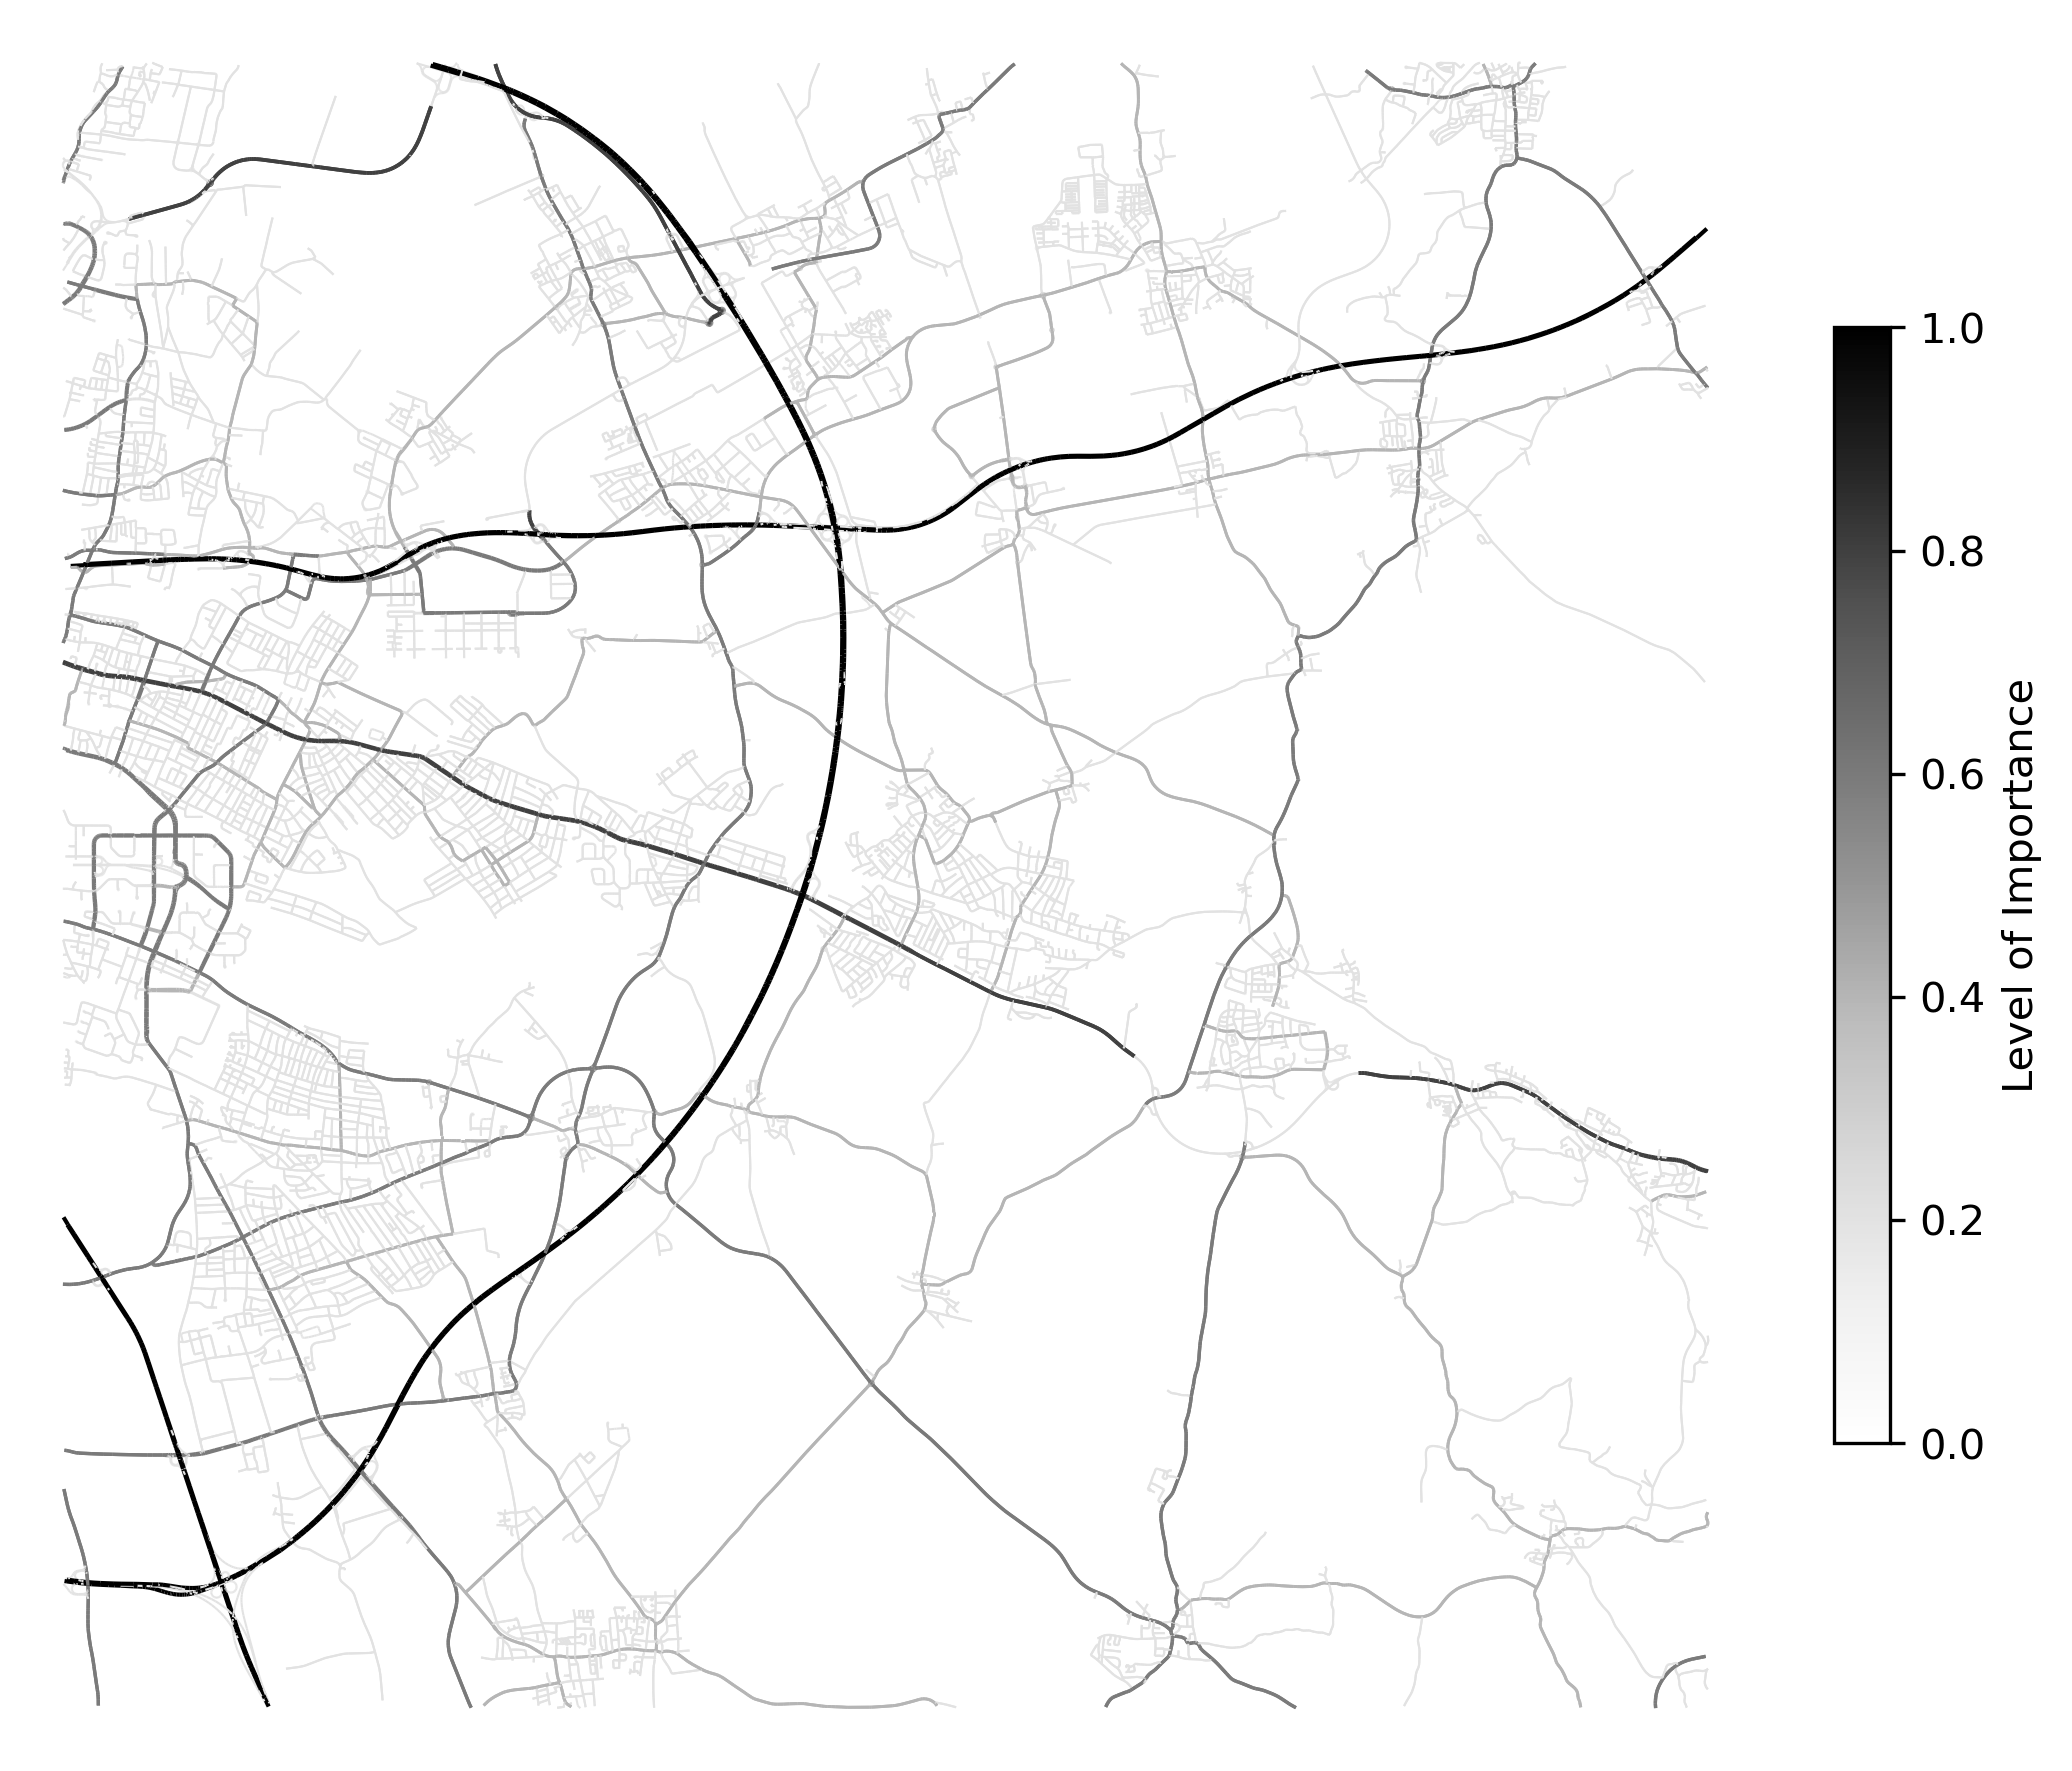
\includegraphics[width=0.5\textwidth]{figures/road_hierarchy.png}
    \caption[Hierarchie in Straßennetzen]{Hierarchie in Straßennetzen. Autobahnen (schwarz) sind ganz oben in der Hierarchie und
        sind sehr "`wichtig"'. Dagegen sind Straßen in Wohnsiedlungen weniger wichtig. \osmcr}
    \label{fig:road_hierarchy}

\end{figure}
\subsubsection{Vorverarbeitung}


\subsubsection{Suche}

\subsection{OpenStreetMap}
OpenStreetMap (OSM) ist ein Projekt, das sich der Erstellung und Bereitstellung von freien
geografischen Daten verschrieben hat. Es handelt sich dabei um Daten die von einer weltweiten
Gemeinschaft von Freiwilligen erstellt und gepflegt wird \cite{osm.about}.

Das grundlegende Konzept von OpenStreetMap basiert auf OpenData, was bedeutet, dass die Daten frei
verfügbar und für jeden zugänglich sind. Im Gegensatz zu kommerziellen Kartenanbietern, die ihre
Daten schützen und für den Zugriff hohe Gebühren verlangen, ermutigt OpenStreetMap Menschen dazu,
ihre eigenen Daten beizutragen und von den vorhandenen Daten zu profitieren.

Das OpenStreetMap-Projekt verwendet eine Kombination aus verschiedenen Datenquellen, um eine
detaillierte und umfassende Karte zu erstellen. Dazu gehören zum Beispiel Satellitenbilder,
GPS-Tracks, Luftaufnahmen und auch öffentlich verfügbare geografische Daten. Die Daten werden von
Freiwilligen erfasst, indem sie Straßen, Gebäude, Gewässer, Landnutzung und andere geografische
Merkmale auf der Karte markieren oder Informationen darüber hinzufügen.

Die OpenStreetMap-Daten sind unter einer offenen Lizenz, der Open Data Commons Open Database Lizenz
(ODbL), verfügbar. Das bedeutet, dass die Daten frei verwendet, kopiert, modifiziert und
weiterverbreitet werden können, solange die Lizenzbedingungen eingehalten werden \cite{osm.license}.
Dadurch wird Entwicklern ermöglicht, die OpenStreetMap-Daten in ihre eigenen Anwendungen und
Dienste zu integrieren.